\documentclass[journal,12pt,twocolumn]{IEEEtran}
\usepackage[utf8]{inputenc}
\usepackage{tabularx}
\usepackage{multicol}
\usepackage{graphicx}
\graphicspath{ {images/} }

\vspace{3cm}
       
\title{AI1100 ASSIGNMENT1} 
\author{AI21BTECH11016} 
\date{March 2022}     
\begin{document}

\maketitle

\textbf{Problem 4-C}\\\\
Draw a circle of radius 4 cm. Mark the centre as O. Mark a point P outside the circle at distance of 7 cm from the centre. Construct two tangents to the circle from the external point P.
Measure and write down the length of any one tangent.\\\\

\textbf{Solution: }
The input parameters for this construction are available in table1.\\

\begin{table}[h]
   \begin{tabular}{|c|c|c|}
   \hline
   \textbf{Symbol} & \textbf{Value} & \textbf{Description}\\
   \hline
   r & $4$ & Radius\\
   \hline
   d & 7 & Distance of P from the centre of circle\\
   \hline
   sin\theta & $r/d$ & Angle b/w the tangent from P and d\\
   \hline
   P & \myvec{(d, 0)} & Point $(0,7)$\\ 
   \hline
   O & \vec{O} & Origin\\
   \hline
   Qi & $rcot\theta \myvec{ (cos\theta, \pm sin\theta)}$ & Points of Contact\\
   \hline
   \end{tabular}\\\\
   \caption{}
   \label{table:1}
\end{table}



\begin{enumerate}


\item Drawing a circle of radius $4 cm$. Taking a point P outside the circle at a distance of $7 cm$ from the centre of the circle and constructing a pair of tangents to the circle from that point using Python. \\


	
  \begin{figure}[h!]
	  \centering 
	  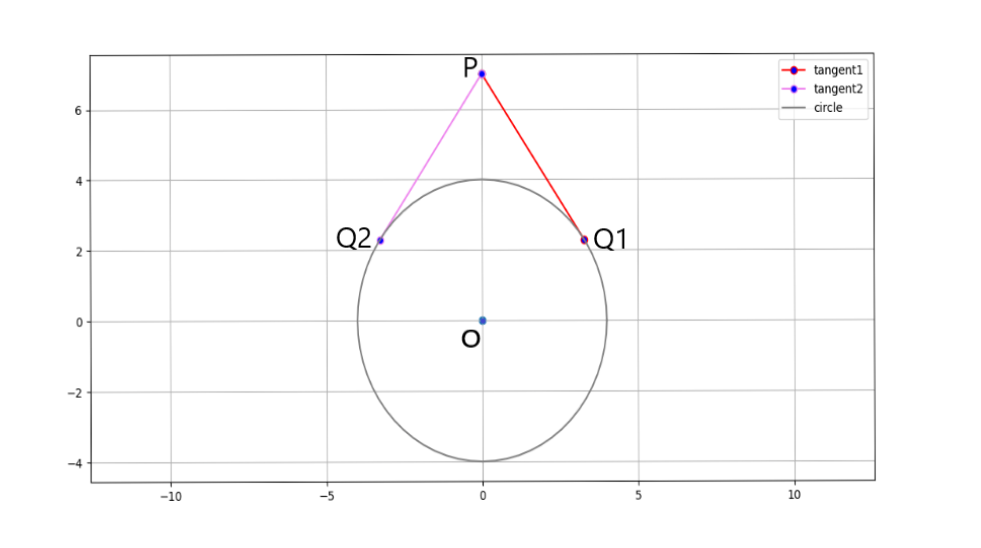
\includegraphics[width=\columnwidth]{imagePython}
	  \caption{}
	  \end{figure}  

\begin{align}

  Consider \triangle OQ2P,\\
    \angle OQ2P = $\Pi/2$,\\
    From Pythogorean Theorem,\\
    \Rightarrow $OP^2 = OQ2^2 + PQ2^2$\\
    OP = 7 and OQ2 = 4\\
    \Rightarrow $PQ2 = \surd33\\\\
    
    \textbf{Therefore, the length of tangent from P is $\surd33$}

\end{align}
 	      

\end{enumerate}

\end{document}

